
\section{数学}
\subsection{整数}
\subsubsection{剰余}
\lstinputlisting{math/modulo/number_theory.cpp}

\subsubsection{カタラン数}
$n\leq 16$程度が限度. $n\geq 1$について以下が成り立つ.
\begin{eqnarray*}
  C_n &=& \frac{1}{n+1}\binom{2n}{n}\\
      &=& \binom{2n}{n}-\binom{2n}{n-1}\\
\end{eqnarray*}
nが十分大きいとき, カタラン数は以下に近似できる.
\begin{eqnarray*}
  C_n &=& \frac{4^n}{n^{3/2}\sqrt{\pi}}\\
\end{eqnarray*}
()を正しく並べる方法, 二分木, 格子状の経路の数え上げ, 平面グラフの交差などに使われる.\\
$C_3=5$\\
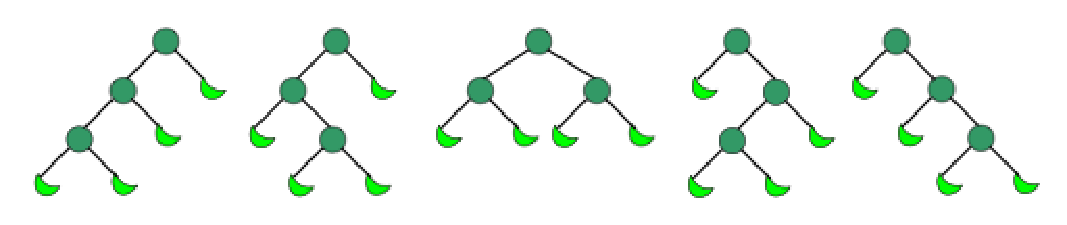
\includegraphics[width=9cm, clip]{images/Catalan_tree.eps}\\
$C_4=14$\\
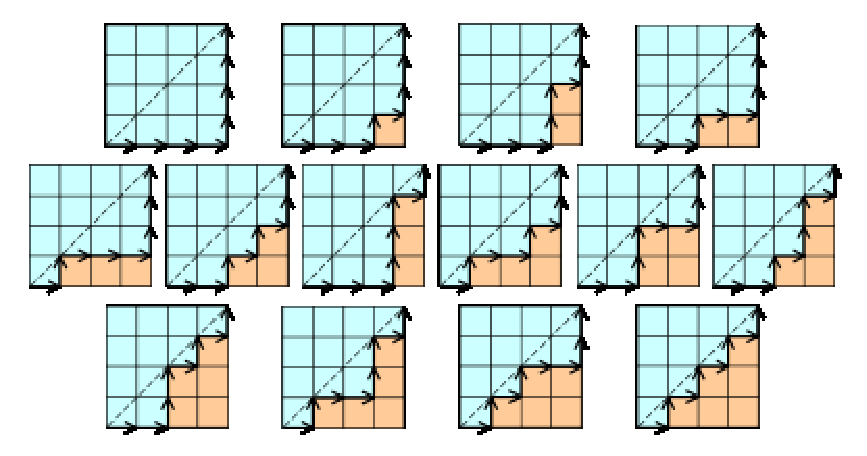
\includegraphics[width=9cm, clip]{images/Catalan_graph.eps}\\

\subsubsection{乱数(xor shift)}
周期は$2^{128}-1$
\lstinputlisting{math/xor_rand.cpp}

\subsubsection{確率的素数判定(Miller-Rabin法)}
$O(k\log^3n)$\par
合成数を素数と判定する確率は最大で$4^{-k}$\\
\lstinputlisting{math/miller_rabin.cpp}

\subsection{多項式}
FFTは基本定数重めなのでTLEに注意する.
\subsubsection{FFT(complex)}
$O(N \log N)$\par
複素数を用いたFFT. 変換するvectorのサイズは2の冪乗にすること.
\lstinputlisting{math/fft.cpp}

\subsubsection{FFT(modulo)}
$O(N \log N)$\par
剰余環を用いたFFT(FMT). 変換するvectorのサイズは2の冪乗にすること. modは$a*2^e+1$の形.\\
\lstinputlisting{math/fmt.cpp}

\subsubsection{積(FMT)}
$O(N \log N)$\par
$poly\_mul()$が必要.
\lstinputlisting{math/poly_mul.cpp}

\subsubsection{逆元(FMT)}
$O(N \log N)$\par
$extgcd()$, $mod\_inverse()$, $poly\_mul()$, $fmt()$が必要.
\lstinputlisting{math/poly_inv.cpp}

\subsubsection{平方根(FMT)}
$O(N log N)$\par
$extgcd()$, $mod\_inverse()$, $poly\_inv()$, $poly\_mul()$, $fmt()$が必要.
\lstinputlisting{math/poly_sqrt.cpp}


\subsection{行列}
\lstinputlisting{math/matrix/matrix.cpp}

\subsubsection{線形方程式の解(Givens消去法)}
$O(N^3)$
\lstinputlisting{math/matrix/givens.cpp}
